% "{'classe':('PSI'),'chapitre':'cin_trans','type':('cours'),'titre':'Transmetteurs de puissance', 'source':'','comp':(''),'corrige':True}"
\setchapterimage{Header_Peugeot.jpg}
\setchapterpreamble[u]{\margintoc}
%\setcounter{chapter}{1}

%\chapter{Transmetteurs de puissance}
\section{Transmetteurs de puissance}

\marginnote[8cm]{
%\UPSTIcompetence[2]{B2-14}
%\UPSTIcompetence[2]{C2-03}
}


\subsection{Transmission par engrenages}
\begin{defi}{Engrenage}
Un engrenage est constitué de deux roues dentées en contact. Une roue dentée est caractérisée (entre autre) par son nombre de dents $Z$, son diamètre primitif $D$ en \si{mm} et son module en \si{mm}. On a $D=mZ$.
Pour que deux dents engrènent elles doivent avoir le même module.
\end{defi}

\subsubsection{Engrenage -- Contact extérieur}
\begin{table*}[!h]
\begin{minipage}[c]{.4\linewidth}
\begin{resultat}
$$
\dfrac{\omega(2/0)}{\omega(1/0)}= (-1)^n \dfrac{Z_1}{Z_2}=-\dfrac{Z_1}{Z_2}
$$
$n$ caractérise le nombre de contacts extérieurs, ici $n=1$.
\end{resultat}
\end{minipage}\hfill
\begin{minipage}[c]{.6\linewidth}
\begin{center}
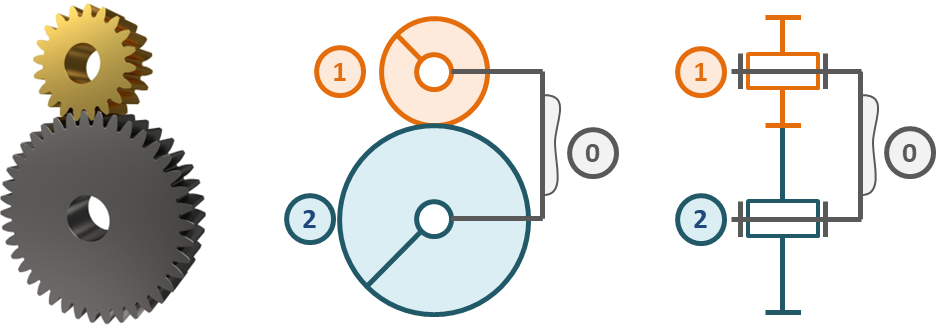
\includegraphics[height=3cm]{fig_01.png}
\end{center}
\end{minipage}
\end{table*}

\newpage

\subsubsection{Engrenage -- Contact intérieur}
\begin{table*}[!h]
\begin{minipage}[c]{.4\linewidth}
\begin{resultat}
$$
\dfrac{\omega(2/0)}{\omega(1/0)}= (-1)^n \dfrac{Z_1}{Z_2}=+\dfrac{Z_1}{Z_2}
$$
$n$ caractérise le nombre de contacts extérieurs, ici $n=0$.
\end{resultat}
\end{minipage}\hfill
\begin{minipage}[c]{.6\linewidth}
\begin{center}
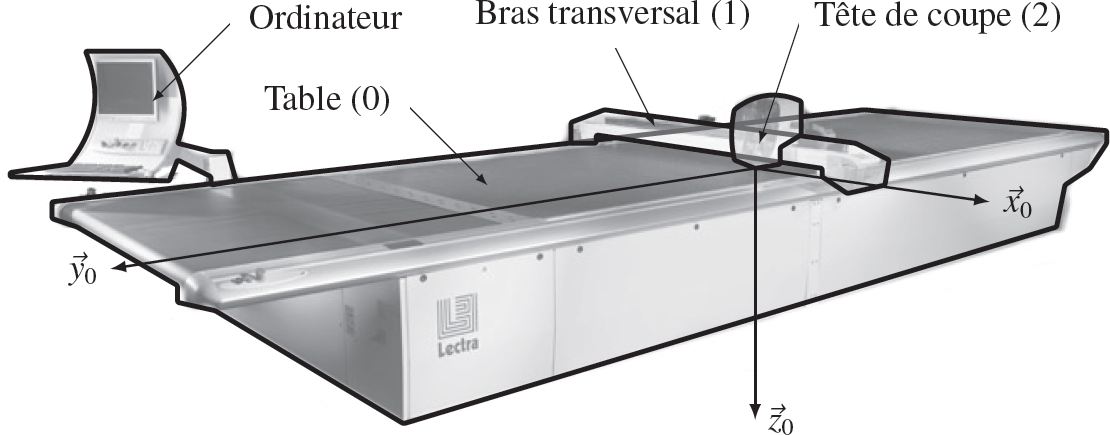
\includegraphics[height=3cm]{fig_02.png}
\end{center}
\end{minipage}
\end{table*}

\subsubsection{Train d'engrenages à axes fixes}


\begin{resultat}
$$
\dfrac{\omega(4/0)}{\omega(1/0)}= (-1)^n \dfrac{\Pi Z_{\text{menantes}}}{\Pi Z_{\text{menées}}}=-\dfrac{Z_1Z_{22}}{Z_{21}Z_4}
$$
$n$ caractérise le nombre de contacts extérieurs, ici $n=1$.
\end{resultat}


\begin{marginfigure}[-4cm]
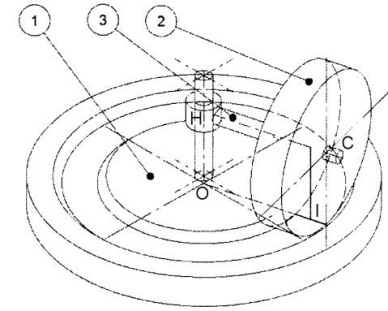
\includegraphics[width=\linewidth]{fig_06.png}
\end{marginfigure}



\subsubsection{Train d'engrenages épicycloïdal}
\begin{marginfigure}
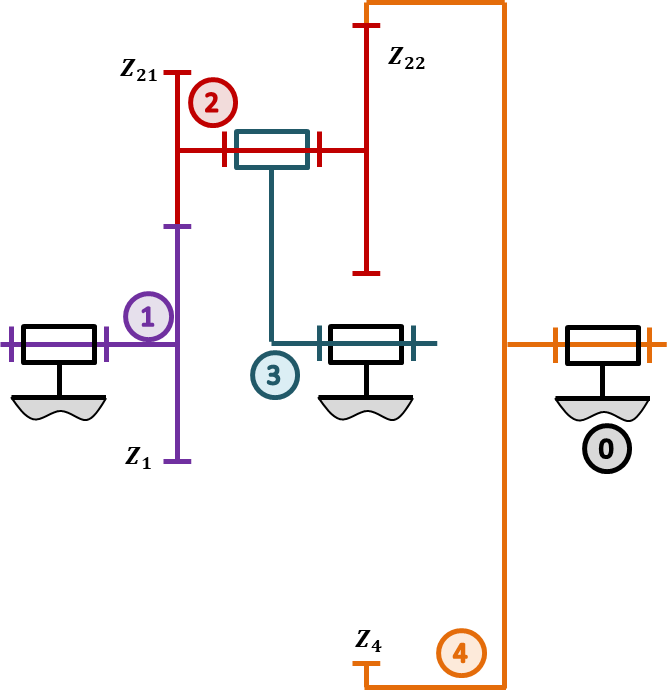
\includegraphics[width=\linewidth]{fig_05.png}
\end{marginfigure}

%\begin{minipage}[c]{.65\linewidth}
\begin{methode}
\begin{enumerate}
\item On identifie le porte-satellite, ici 3.
\item On bloque le porte-satellite. On peut alors se ramener au cas du train simple (voir ci-dessus). 
\item On écrit le rapport de vitesse \textbf{par rapport au porte-satelltite 3} :$
\dfrac{\omega(4/3)}{\omega(1/3)}=-\dfrac{Z_1Z_{22}}{Z_{21}Z_4} = K
$ (raison du train épicycloïdal).
\item En fonction de la roue bloquée, on réalise une décomposition des vitesses. Par exemple, Si 4 est bloquée, on   peut chercher à établir $\dfrac{\omega(3/0)}{\omega(1/0)}$. 
\item On repart du point 3 et on a : $\dfrac{\omega(4/3)}{\omega(1/3)}= K$
$\Leftrightarrow \dfrac{\omega(4/0)+\omega(0/3)}{\omega(1/0)+\omega(0/3)}= K$
$\Leftrightarrow \dfrac{-\omega(3/0)}{\omega(1/0)-\omega(3/0)}= K$
%$\Leftrightarrow -\omega(3/0) = K\omega(1/0)-K\omega(3/0)$
%$\Leftrightarrow \left(K-1\right)\omega(3/0) = K\omega(1/0)$
$\Leftrightarrow \dfrac{\omega(3/0)}{\omega(1/0)} = \dfrac{K}{K-1}$.
\end{enumerate}
\end{methode}
%\end{minipage}\hfill
%\begin{minipage}[c]{.35\linewidth}
%\begin{center}
%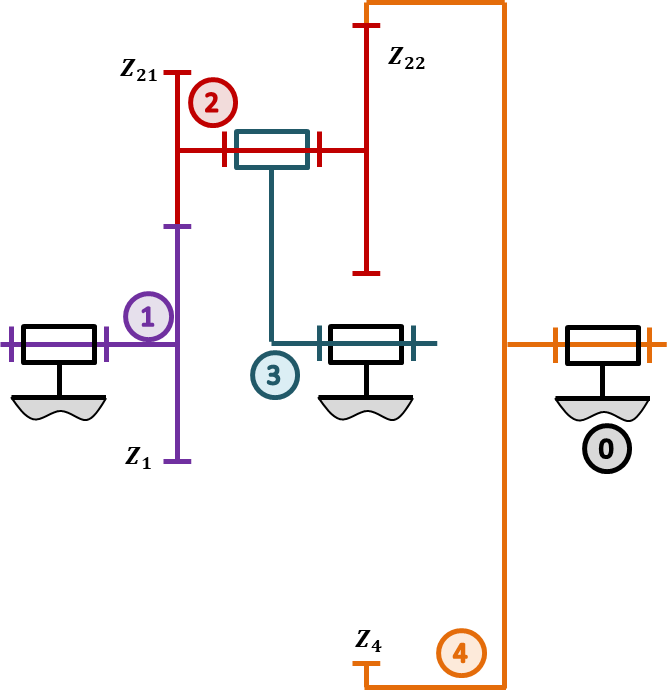
\includegraphics[height=4.5cm]{fig_05.png}
%\end{center}
%\end{minipage}
%
\subsubsection{Système pignon -- crémaillère}

\begin{marginfigure}
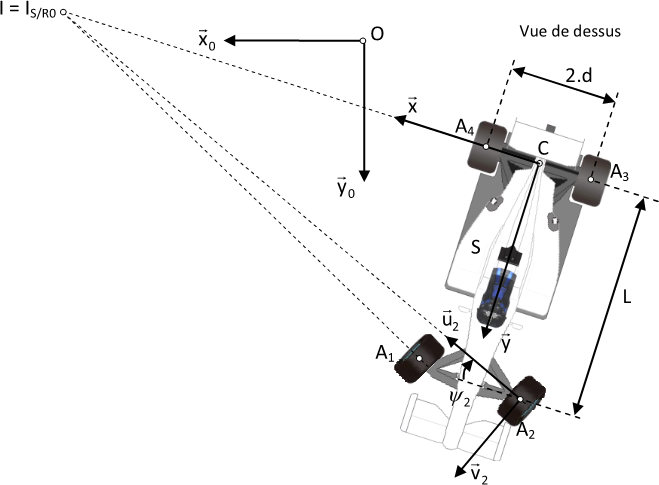
\includegraphics[width=\linewidth]{fig_03.png}
\end{marginfigure}

%\begin{minipage}[c]{.4\linewidth}
\begin{resultat}
Soit $R$ le rayon primitif du pignon. On a $V(2/0) = \pm R \omega(1/0)$.
\end{resultat}
%\end{minipage}\hfill
%\begin{minipage}[c]{.6\linewidth}
%\end{minipage}

\subsubsection{Transmission par poulie chaine et par poulie courroie}
\begin{table*}[!h]
\begin{minipage}[c]{.6\linewidth}
\begin{center}
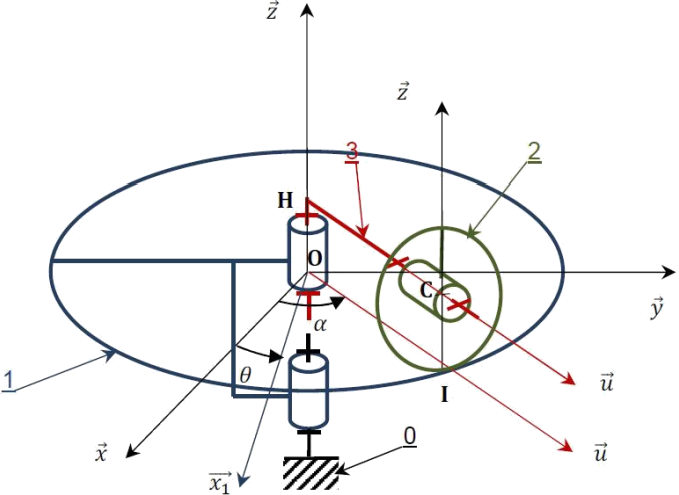
\includegraphics[height=3cm]{fig_07.png}
\end{center}
\end{minipage}\hfill
\begin{minipage}[c]{.4\linewidth}
\begin{resultat}

$\dfrac{\omega(2/0)}{\omega(1/0)} = \dfrac{D_1}{D_2}$.
\end{resultat}
\end{minipage}
\end{table*}

\newpage

\subsubsection{Roue et vis sans fin}
\begin{table*}[!h]
\begin{minipage}[c]{.4\linewidth}
\begin{resultat}
Soit $Z$ le nombre de dents de la roue et $n$ le nombre de filets de la vis, on a 
$\dfrac{\omega(2/0)}{\omega(1/0)} = \pm \dfrac{n}{Z}$.
\end{resultat}
\end{minipage}\hfill
\begin{minipage}[c]{.6\linewidth}
\begin{center}
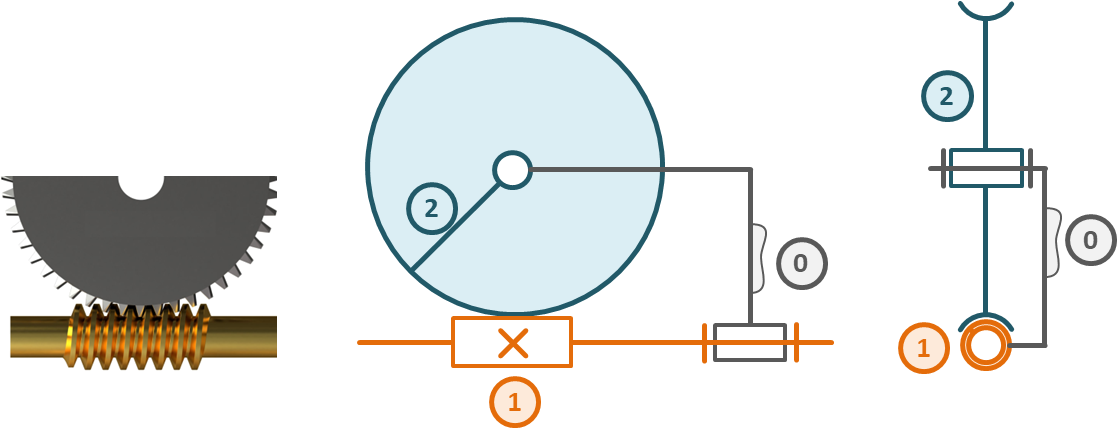
\includegraphics[height=3cm]{fig_04.png}
\end{center}
\end{minipage}
\end{table*}


\subsubsection{Système vis-écrou}
\begin{resultat}
En notant $v$ la vis et $e$ l'écrou, soit $p$ le pas de la vis (ici à droite) on a 
$$v(v/e)=\omega(v/e) \dfrac{\text{pas}}{2 \pi}$$.
\end{resultat}

\subsubsection{Système de transmission Rotation -- Rotation}
\begin{table*}[!h]
\begin{tabular}{lccc}
\cline{2-4}
& Joint de Oldham & Joint de cardan & Joint tripode \\ \cline{2-4}
\cline{2-4}
&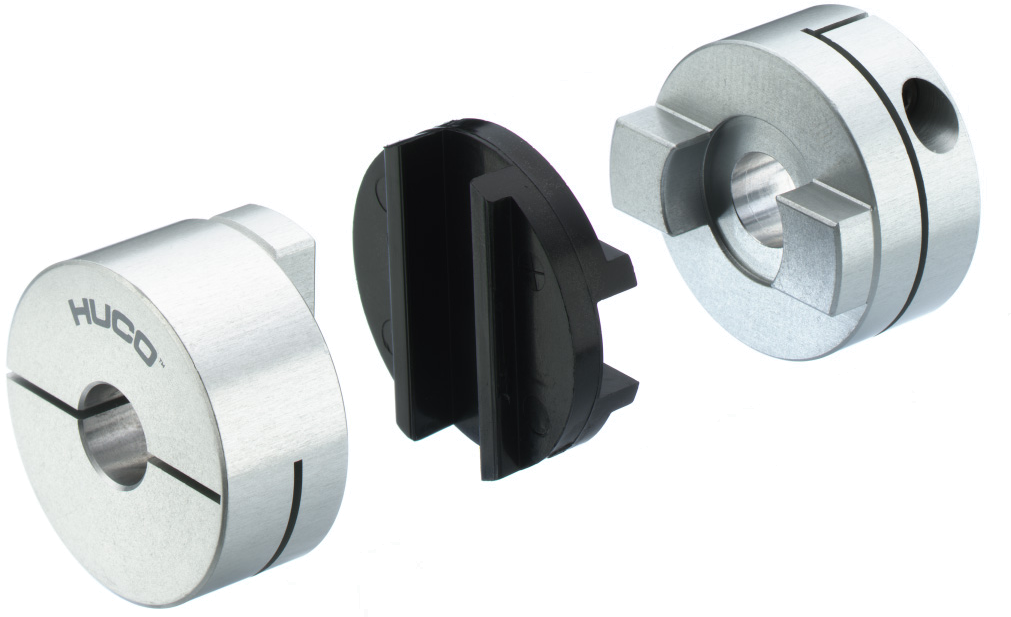
\includegraphics[width=3cm]{fig_08.png}&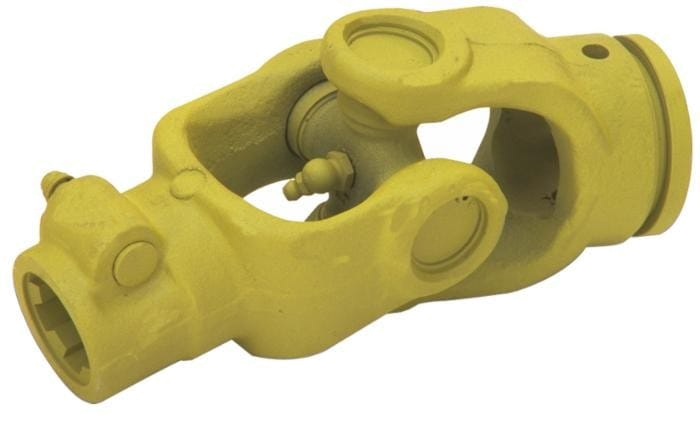
\includegraphics[width=3cm]{fig_09.png}& 
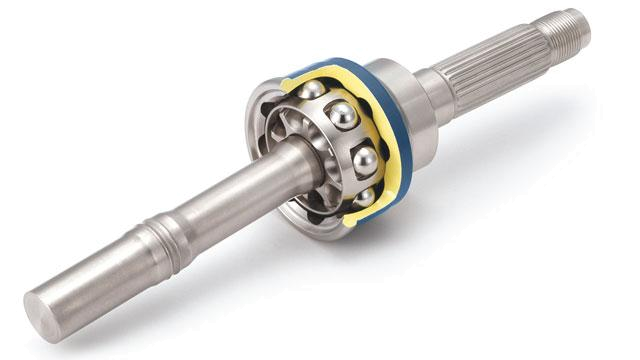
\includegraphics[width=3cm]{fig_10.png}\\ \hline
Homcinétique & Oui & Non, Oui si doublé & Quasi \\ %\hline
Défaut d'alignement axial & Oui & Non & Non \\ %\hline
Défaut d'orientation & \multirow{2}{*}{Non} &  \multirow{2}{*}{Oui}& \multirow{2}{*}{Oui} \\ 
entre les axes  & & & \\ %\hline 
 & & Colonne de & \\
Utilsation&Maxpid :) &  direction (DAE),  & Automobile \\
&&  manivelle de volet roulant & \\
\hline
\end{tabular}
\end{table*}
